\documentclass{article}

%Packages and other options are for bells and whistles!
% \usepackage[margin = 1in]{geometry}
% \usepackage{amsmath}
 
\usepackage{Sweave}
\begin{document}

%Need this to make a Sweave document!
\Sconcordance{concordance:STAT673HW0.tex:STAT673HW0.Rnw:%
1 6 1 1 0 14 1 1 2 1 0 2 1 4 0 1 2 2 1 1 2 1 0 6 1 4 0 1 2 2 1 1 2 7 0 %
1 2 5 1 1 2 15 0 1 1 1 2 7 0 1 1 8 0 1 2 13 1}


\begin{flushleft}

Name 1\\
Name 2 \\
STAT 673 Homework \#0\\
\vspace*{2\baselineskip}
%or can use 
%\bigskip
Problem 1 from Lab\\
Part A\\
\begin{Schunk}
\begin{Sinput}
> set.seed(1)
> bindat <- rbinom(n=10000, size=10, prob=0.8)
> hist(bindat, breaks=seq(2, 10, 1), freq=F)
\end{Sinput}
\end{Schunk}
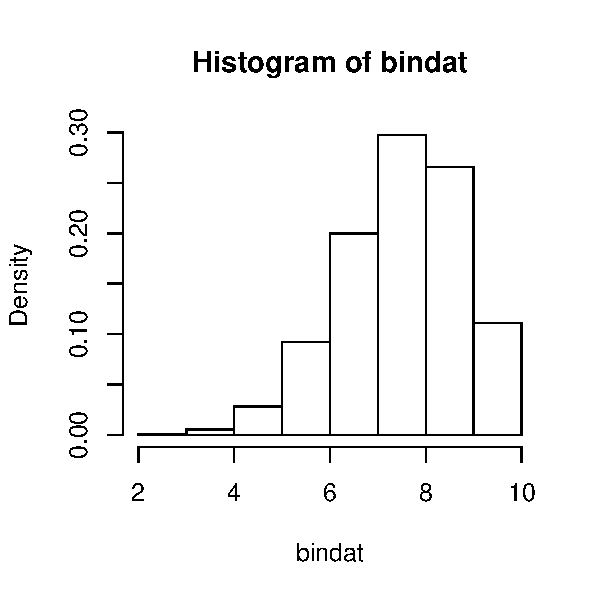
\includegraphics{STAT673HW0-1a}

Let's make a multiple plots in a figure!

\begin{Schunk}
\begin{Sinput}
> set.seed(1)
> bindat <- rbinom(n=10000, size=10, prob=0.8)
> par(mfrow=c(2,2))
> hist(bindat, breaks=seq(2, 10, 1), freq=F)
> hist(bindat, breaks=seq(2, 10, 1), freq=F)
> hist(bindat, breaks=seq(2, 10, 1), freq=F)
> hist(bindat, breaks=seq(2, 10, 1), freq=F)
\end{Sinput}
\end{Schunk}
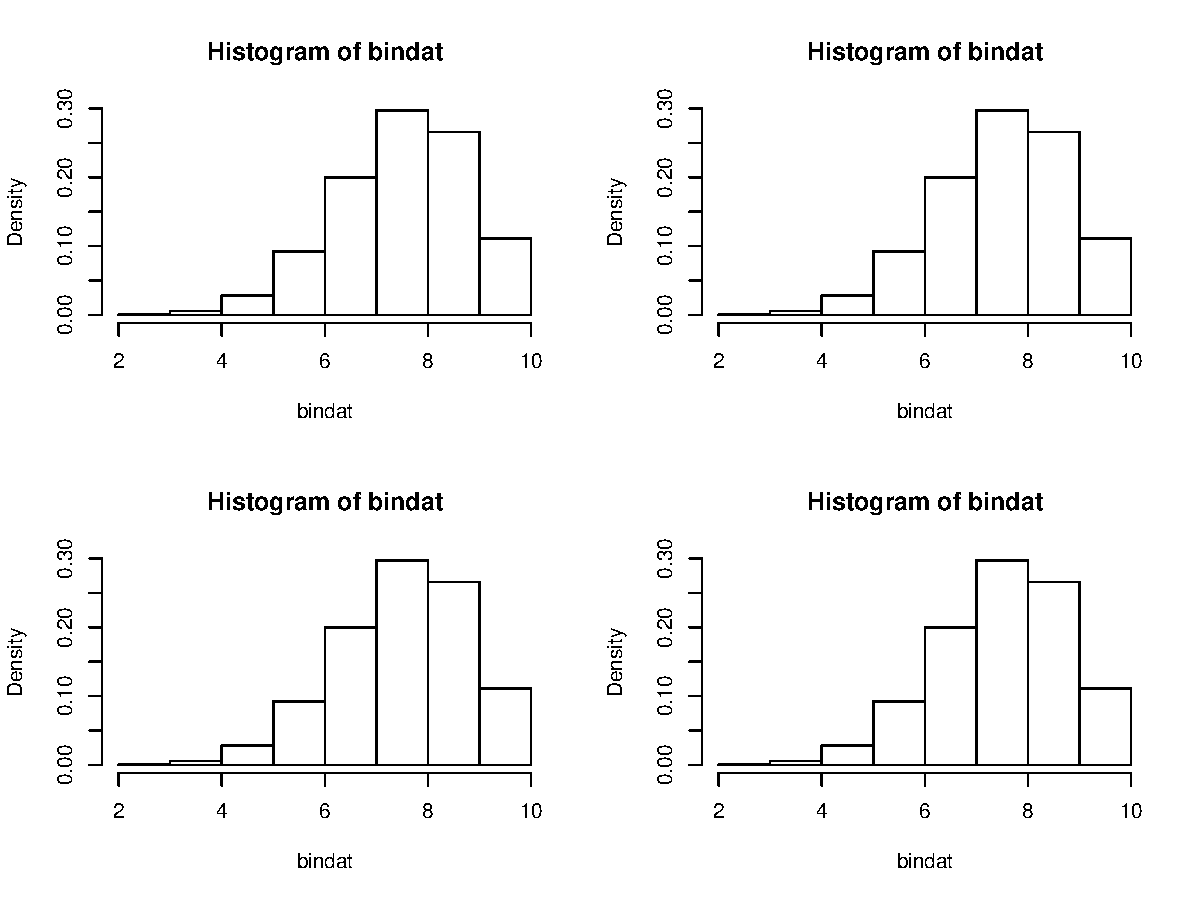
\includegraphics{STAT673HW0-1a2}


Part B\\
\begin{Schunk}
\begin{Sinput}
> 1-pbinom(7, 10, 0.8)
\end{Sinput}
\begin{Soutput}
[1] 0.6777995
\end{Soutput}
\end{Schunk}

The probability that Dr. Dribble makes at least 8 out 10 free throws is 0.6778. 

\pagebreak

Part C\\
\begin{Schunk}
\begin{Sinput}
> binom.test(15, 25, 0.4, alternative="greater")
\end{Sinput}
\begin{Soutput}
	Exact binomial test

data:  15 and 25
number of successes = 15, number of trials = 25, p-value = 0.03439
alternative hypothesis: true probability of success is greater than 0.4
95 percent confidence interval:
 0.416838 1.000000
sample estimates:
probability of success 
                   0.6 
\end{Soutput}
\begin{Sinput}
> hold <- binom.test(15, 25, 0.4, alternative="greater")
> #the names command is useful!
> names(hold)
\end{Sinput}
\begin{Soutput}
[1] "statistic"   "parameter"   "p.value"     "conf.int"    "estimate"   
[6] "null.value"  "alternative" "method"      "data.name"  
\end{Soutput}
\begin{Sinput}
> hold$conf.int
\end{Sinput}
\begin{Soutput}
[1] 0.416838 1.000000
attr(,"conf.level")
[1] 0.95
\end{Soutput}
\end{Schunk}

The hypothesis testing problem is \\
\smallskip
$H_0: p = 0.4$ versus  $H_1: p > 0.4$\\
%\vspace*{1\baselineskip}
\medskip
With a p-value of 0.03439 we reject the null hypothesis. We conclude that there is evidence that the first serve percentage is not 0.4 in favor of the alternative. 
(This is if a tennis player actually makes 15/25 first serves.) \\
\bigskip
You can also interpret the confidence interval!

\end{flushleft}

\end{document}
